  \begin{tikzpicture}[font=\bf\sffamily\fontsize{8}{9}\selectfont]
  \def\DCOL{MediumBlue!40}
  \def\DCOLx{MediumBlue!40}
  %\def\DCOL{Red1}
  %\def\DCOLx{Red1}
  \def\DCOLS{black}
  \def\ECOLA{black!5}
  \def\ECOLB{black!5}
  \def\ECOLC{Green4!5}
  \def\ECOLD{Green4!5}
  \def\LWD{2pt}
  \def\LWDA{6pt}
  \def\ACOL{black}
  \def\OPC{.8}
  \def\OPCA{.95}
  \def\OPCB{.15}
  \def\CIRC{circle}
  \def\SCALE{.80}
  \def\LCOL{black!50}
\node[anchor=south west] (T) at (0,0) {
\includegraphics[width=3in]{Figures/\EPATH}};

\node[anchor=south west,label={[text=black,align=center,yshift=-.6in,xshift=1.5in]120:{\Large b.} A sample of\\conditional inference trees\\in inferred \enet}] at (T.south east) {
  \begin{tikzpicture}[anchor=center,font=\bf\sffamily\fontsize{8}{8}\selectfont]
 \clip (1in,-0.250in) rectangle (-3.05in,-7.15in);
  \tikzset{xcirc/.style={circle,inner sep=-25pt,dashed,fill=\ECOLB,opacity=\OPC,rounded corners=5pt,draw=\DCOL,line width=\LWD,scale=\SCALE}}
    \def\WDT{2.5in}
    \def\WDTA{3.75in}
    \def\WDTB{3.75in}
    \def\WDTC{3in}
    \coordinate (Z) at (0,0);
    \node[anchor=north,xcirc,inner sep=-25pt,label={[yshift=.25in,\LCOL]-90:index 1314}] (P1314) at (Z) {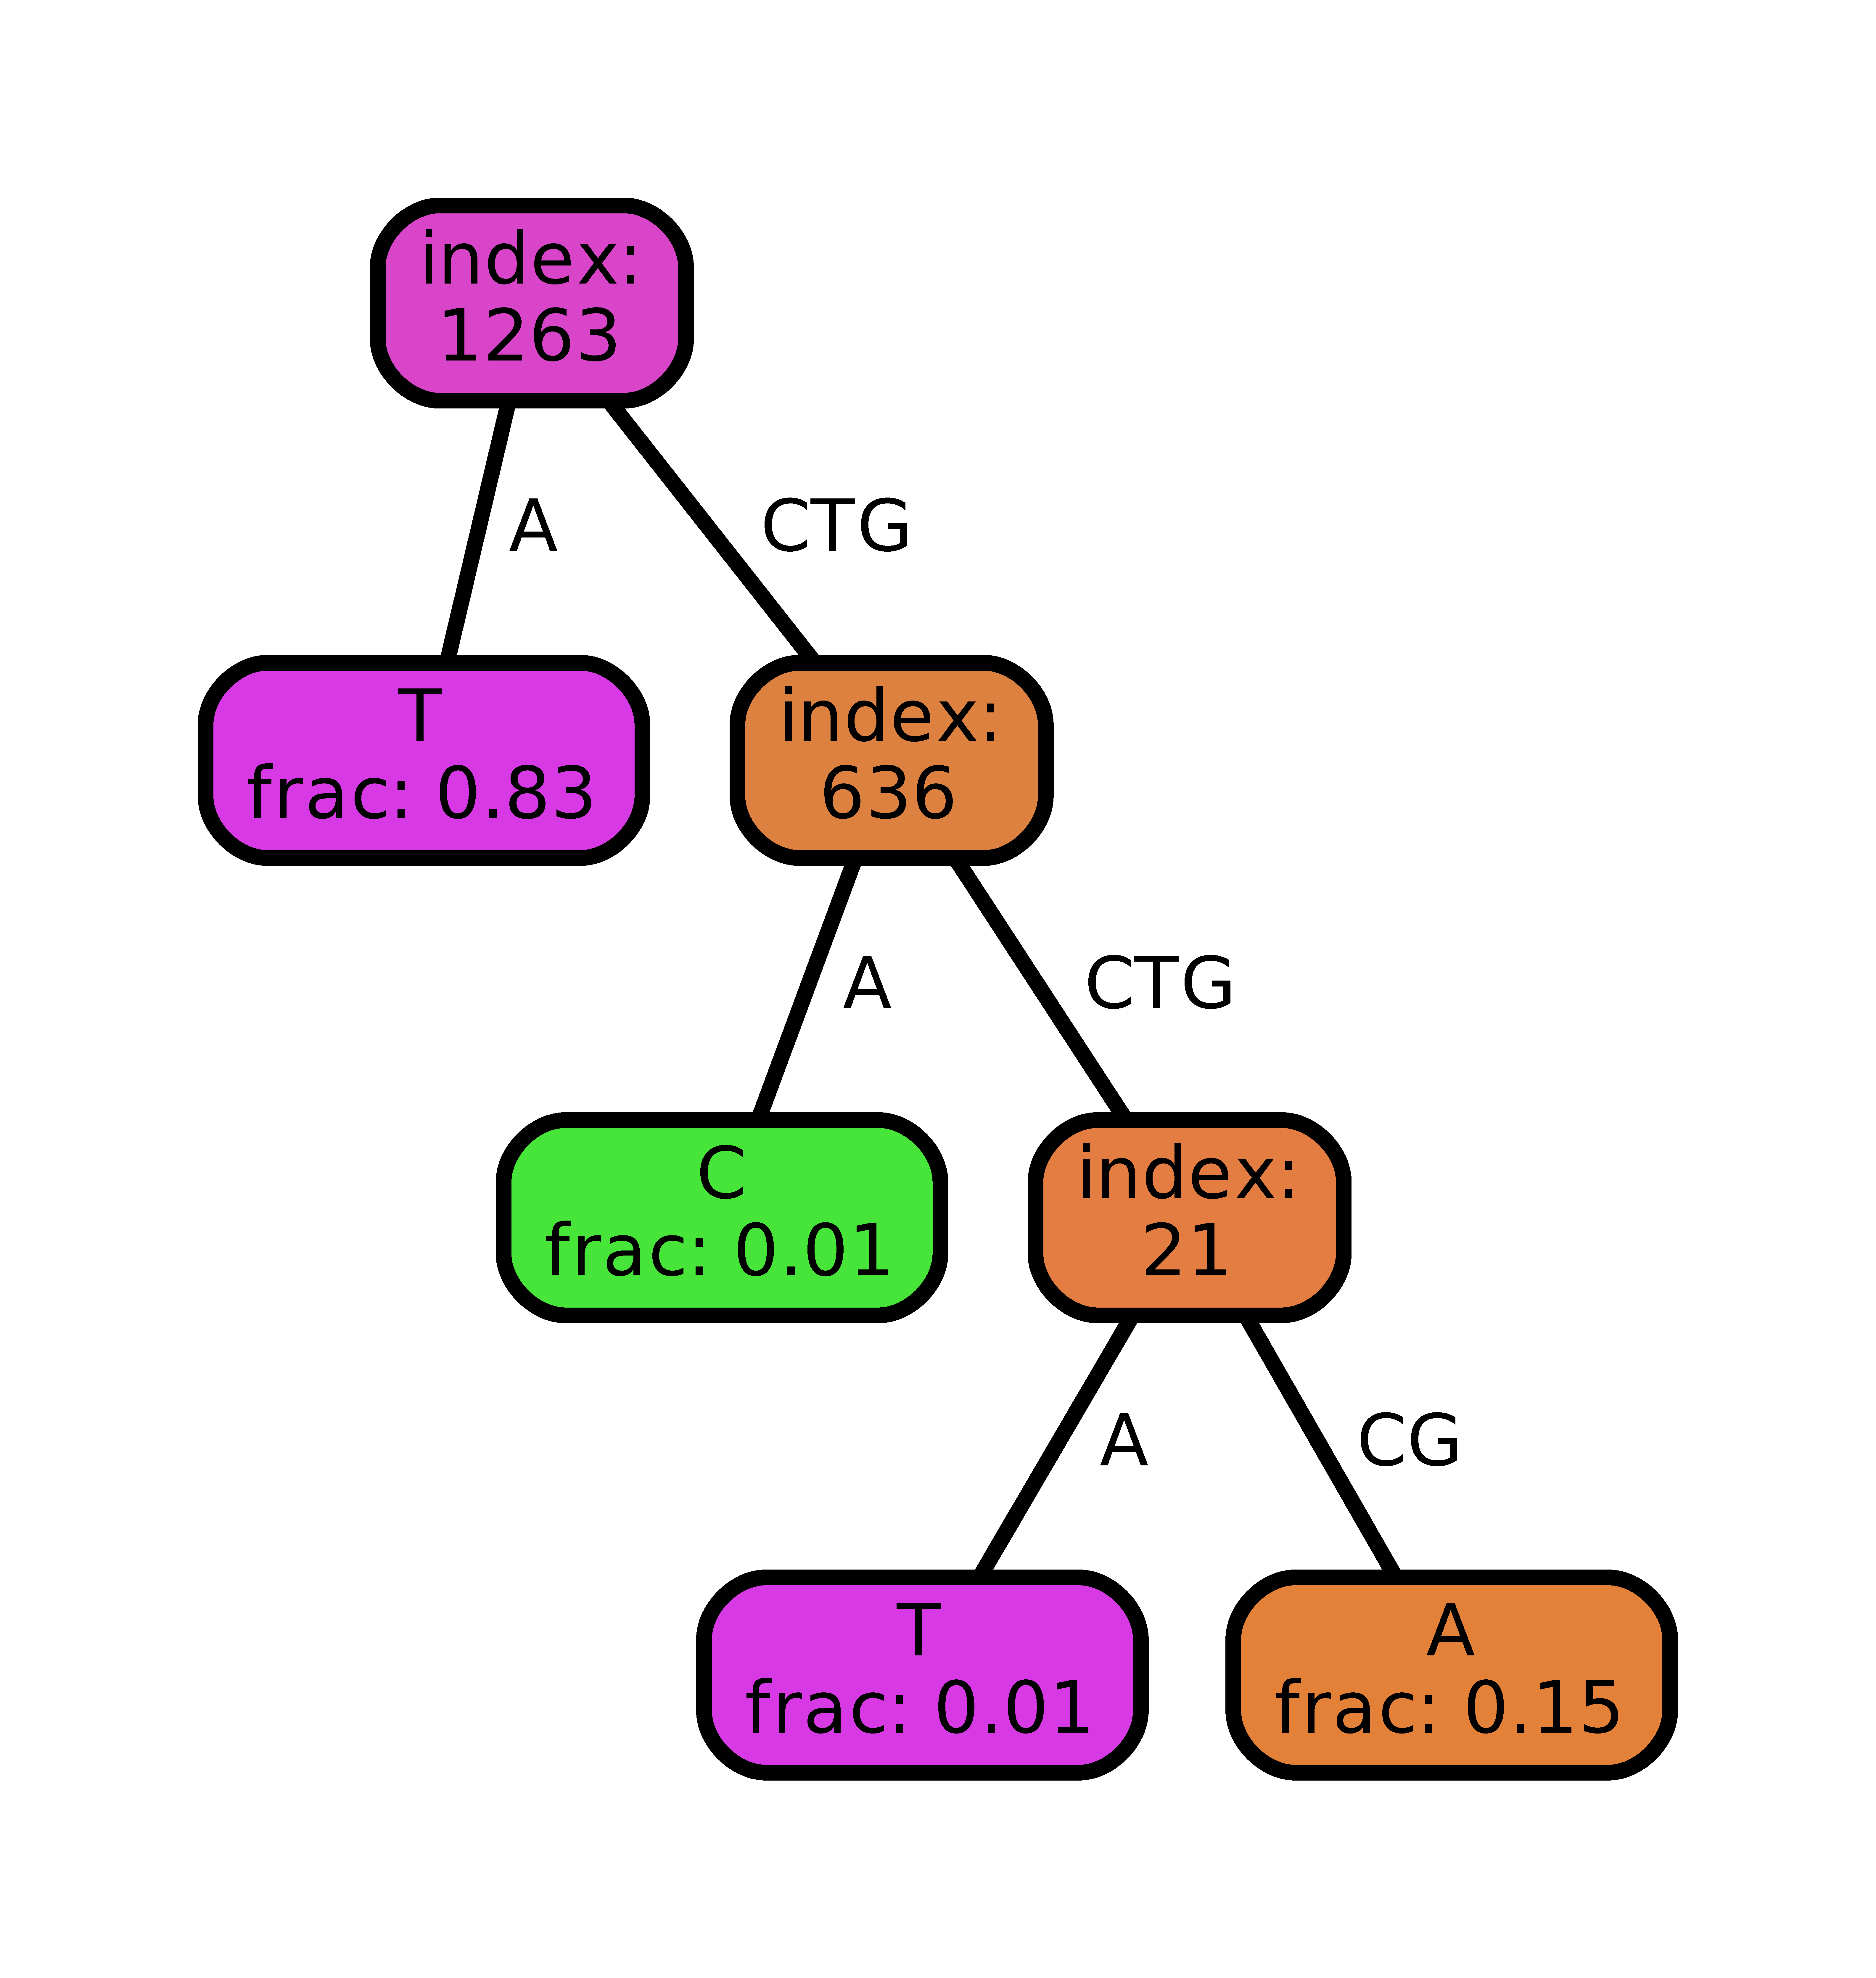
\includegraphics[width=\WDTC]{Figures/trees/procP1314}}; 
    \node[anchor=north,xcirc,inner sep=-30pt,label={[yshift=.4in,\LCOL]-90:index 1274}] (P1274) at ([xshift=-1.5in,yshift=-0.5in]P1314.south) {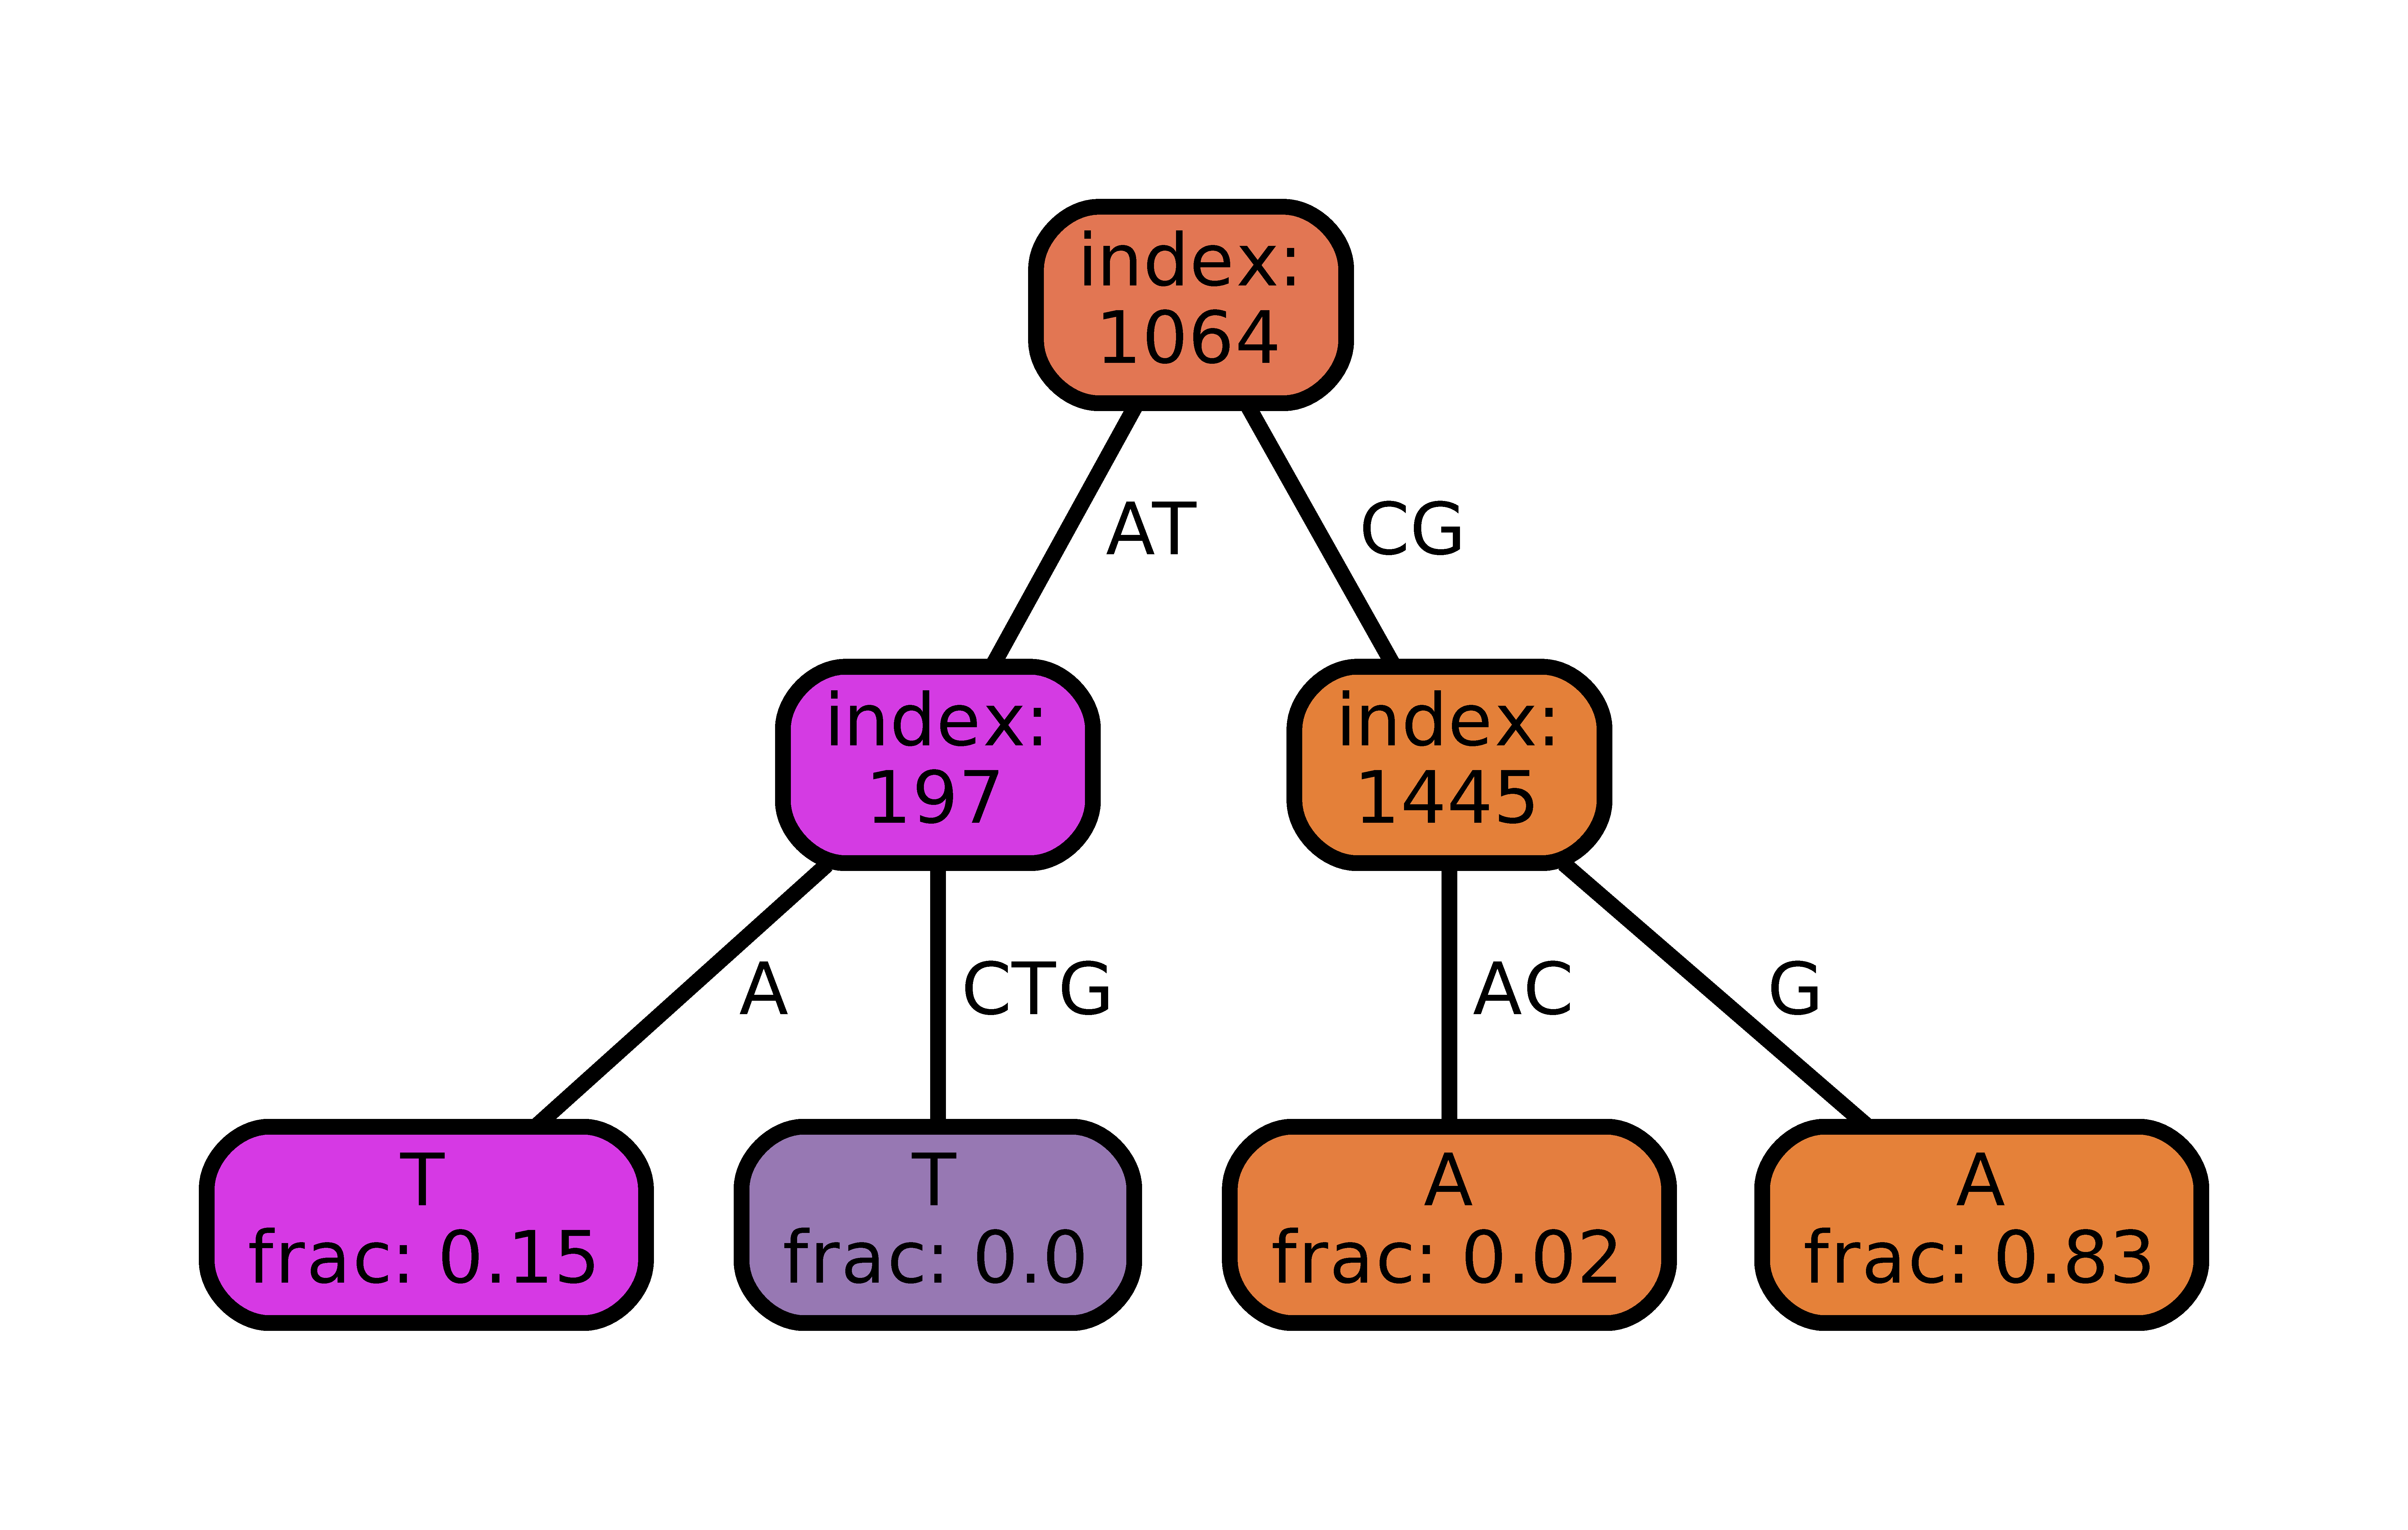
\includegraphics[width=\WDTA]{Figures/trees/procP1274}}; 
    \node[anchor=north west,xcirc,inner sep=-40pt,label={[yshift=.35in,\LCOL]-90:index 1263}] (P1263) at ([xshift=-1.65in,yshift=.85in]P1314.south west) {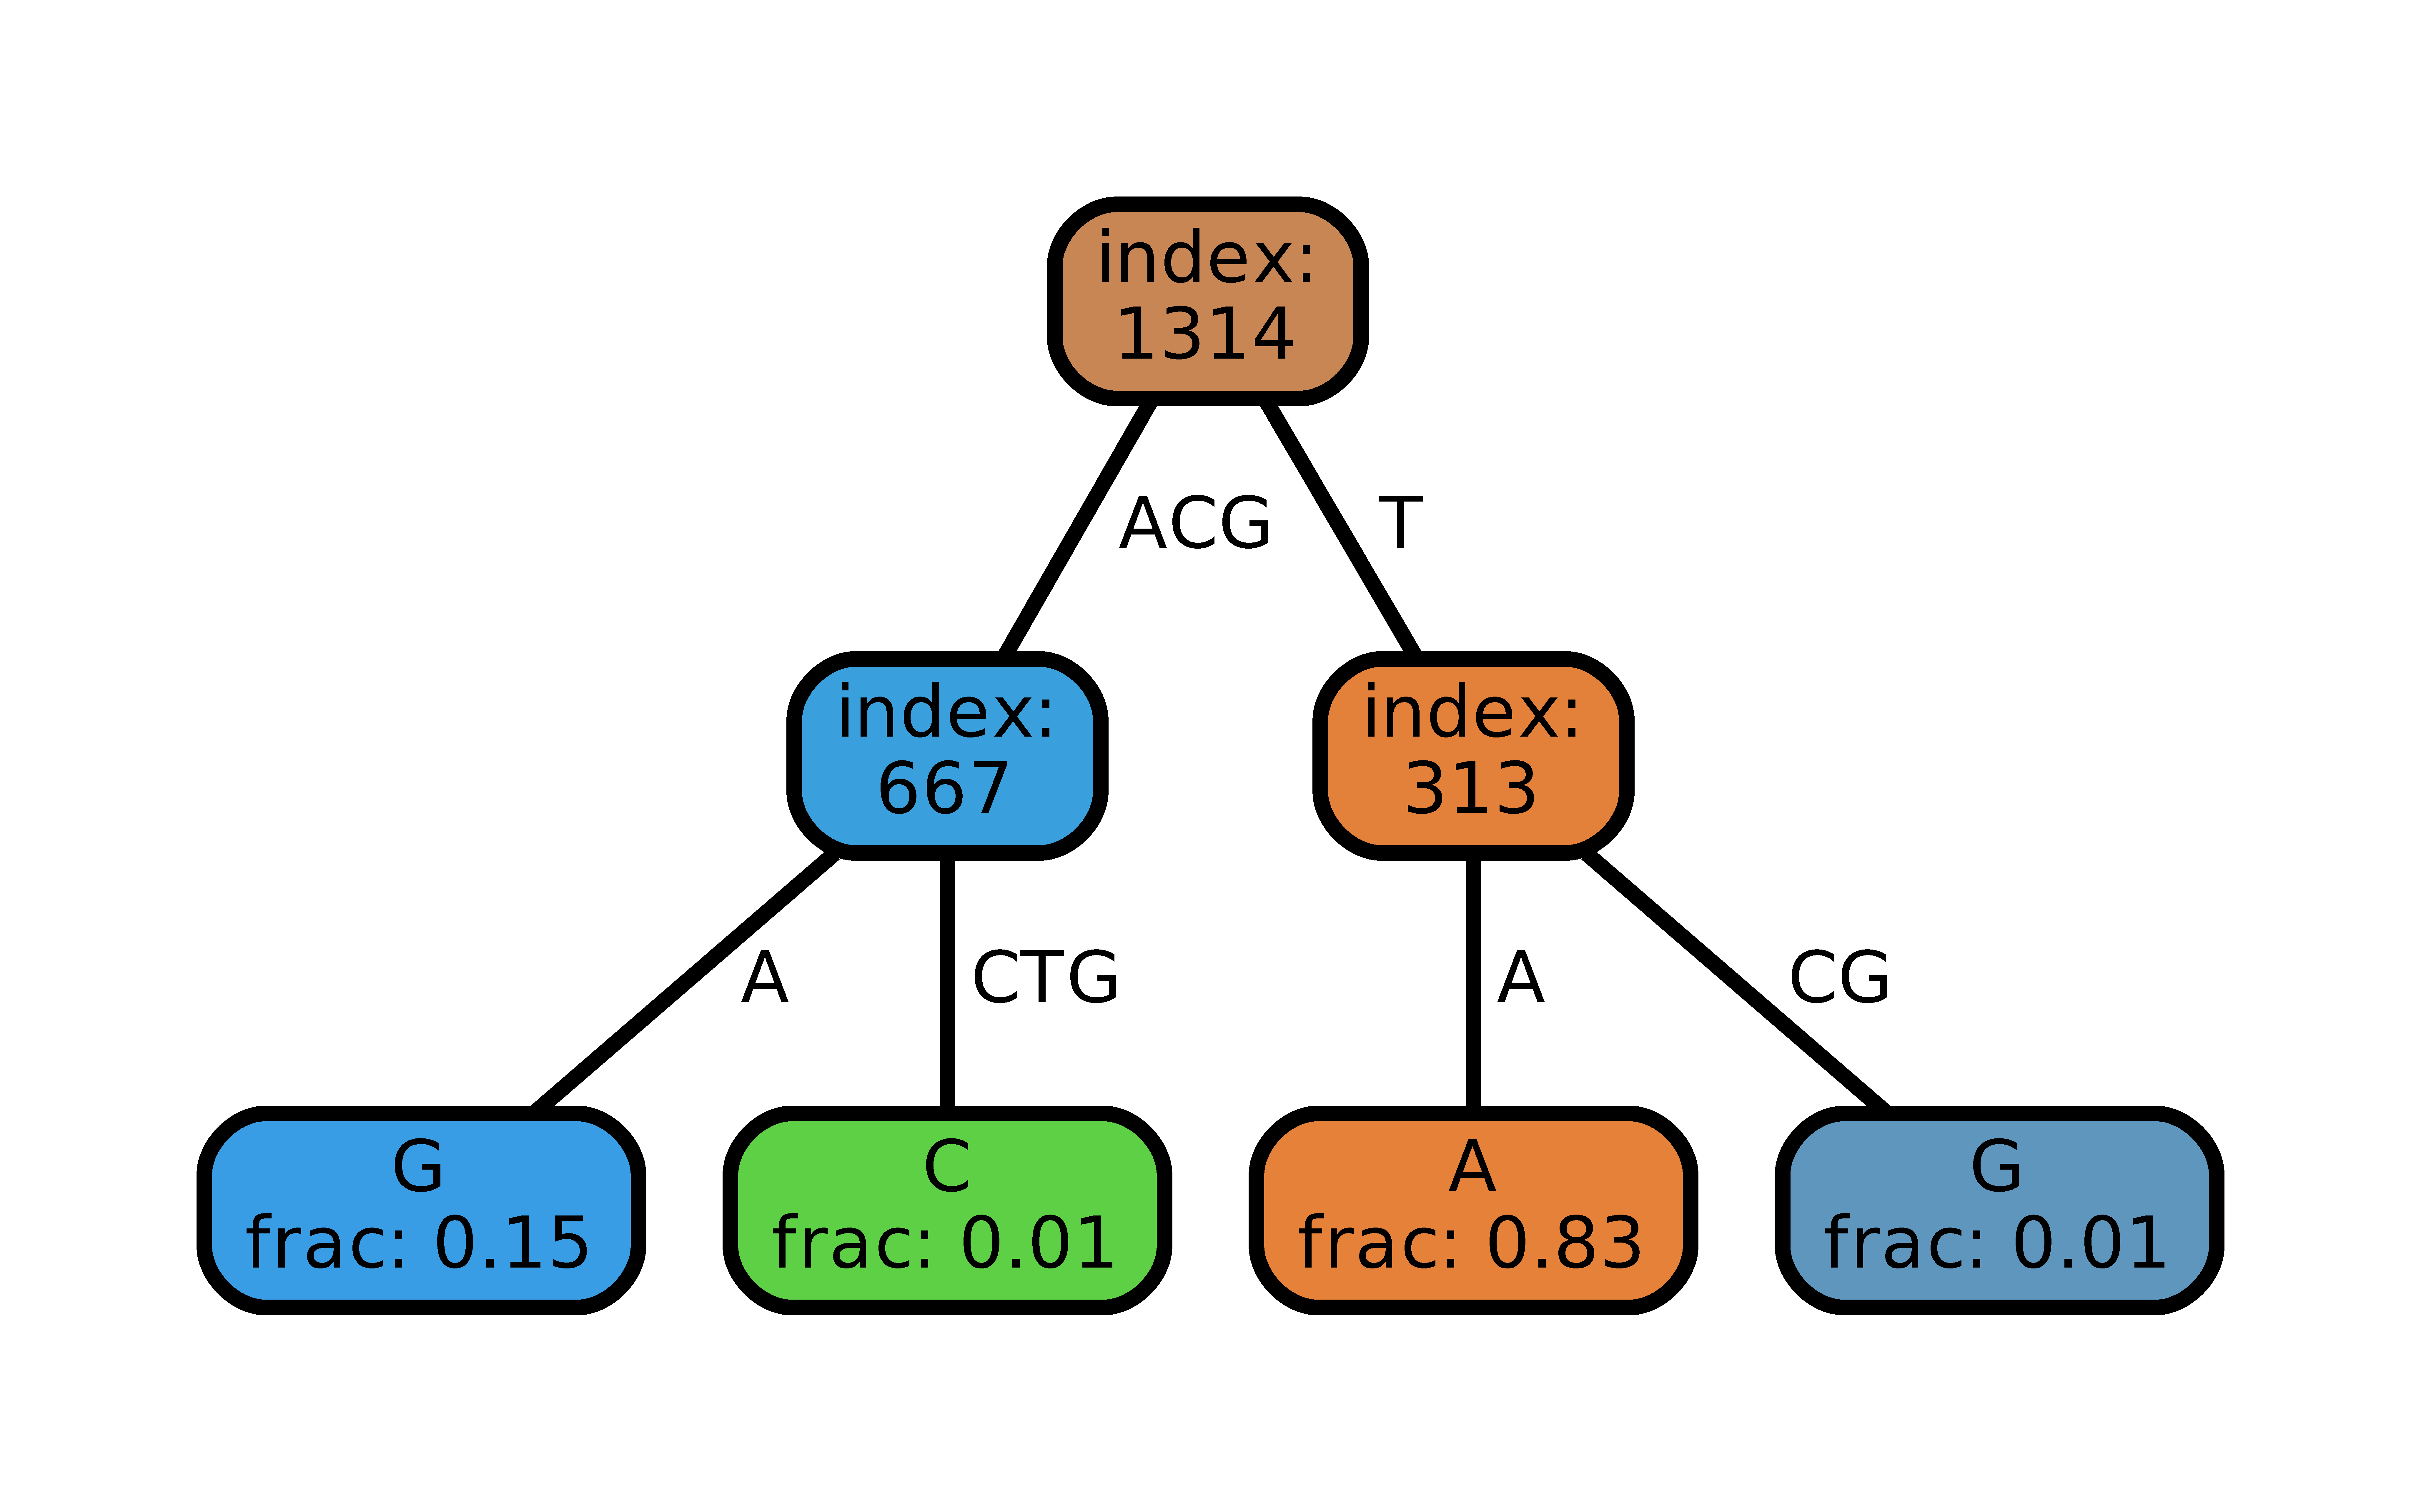
\includegraphics[width=\WDTB]{Figures/trees/procP1263}}; 
    \node[anchor=north,xcirc,label={[yshift=.25in,\LCOL]-90:index 1064}] (P1064) at ([xshift=0.2in,yshift=-0.10in]P1314.south) {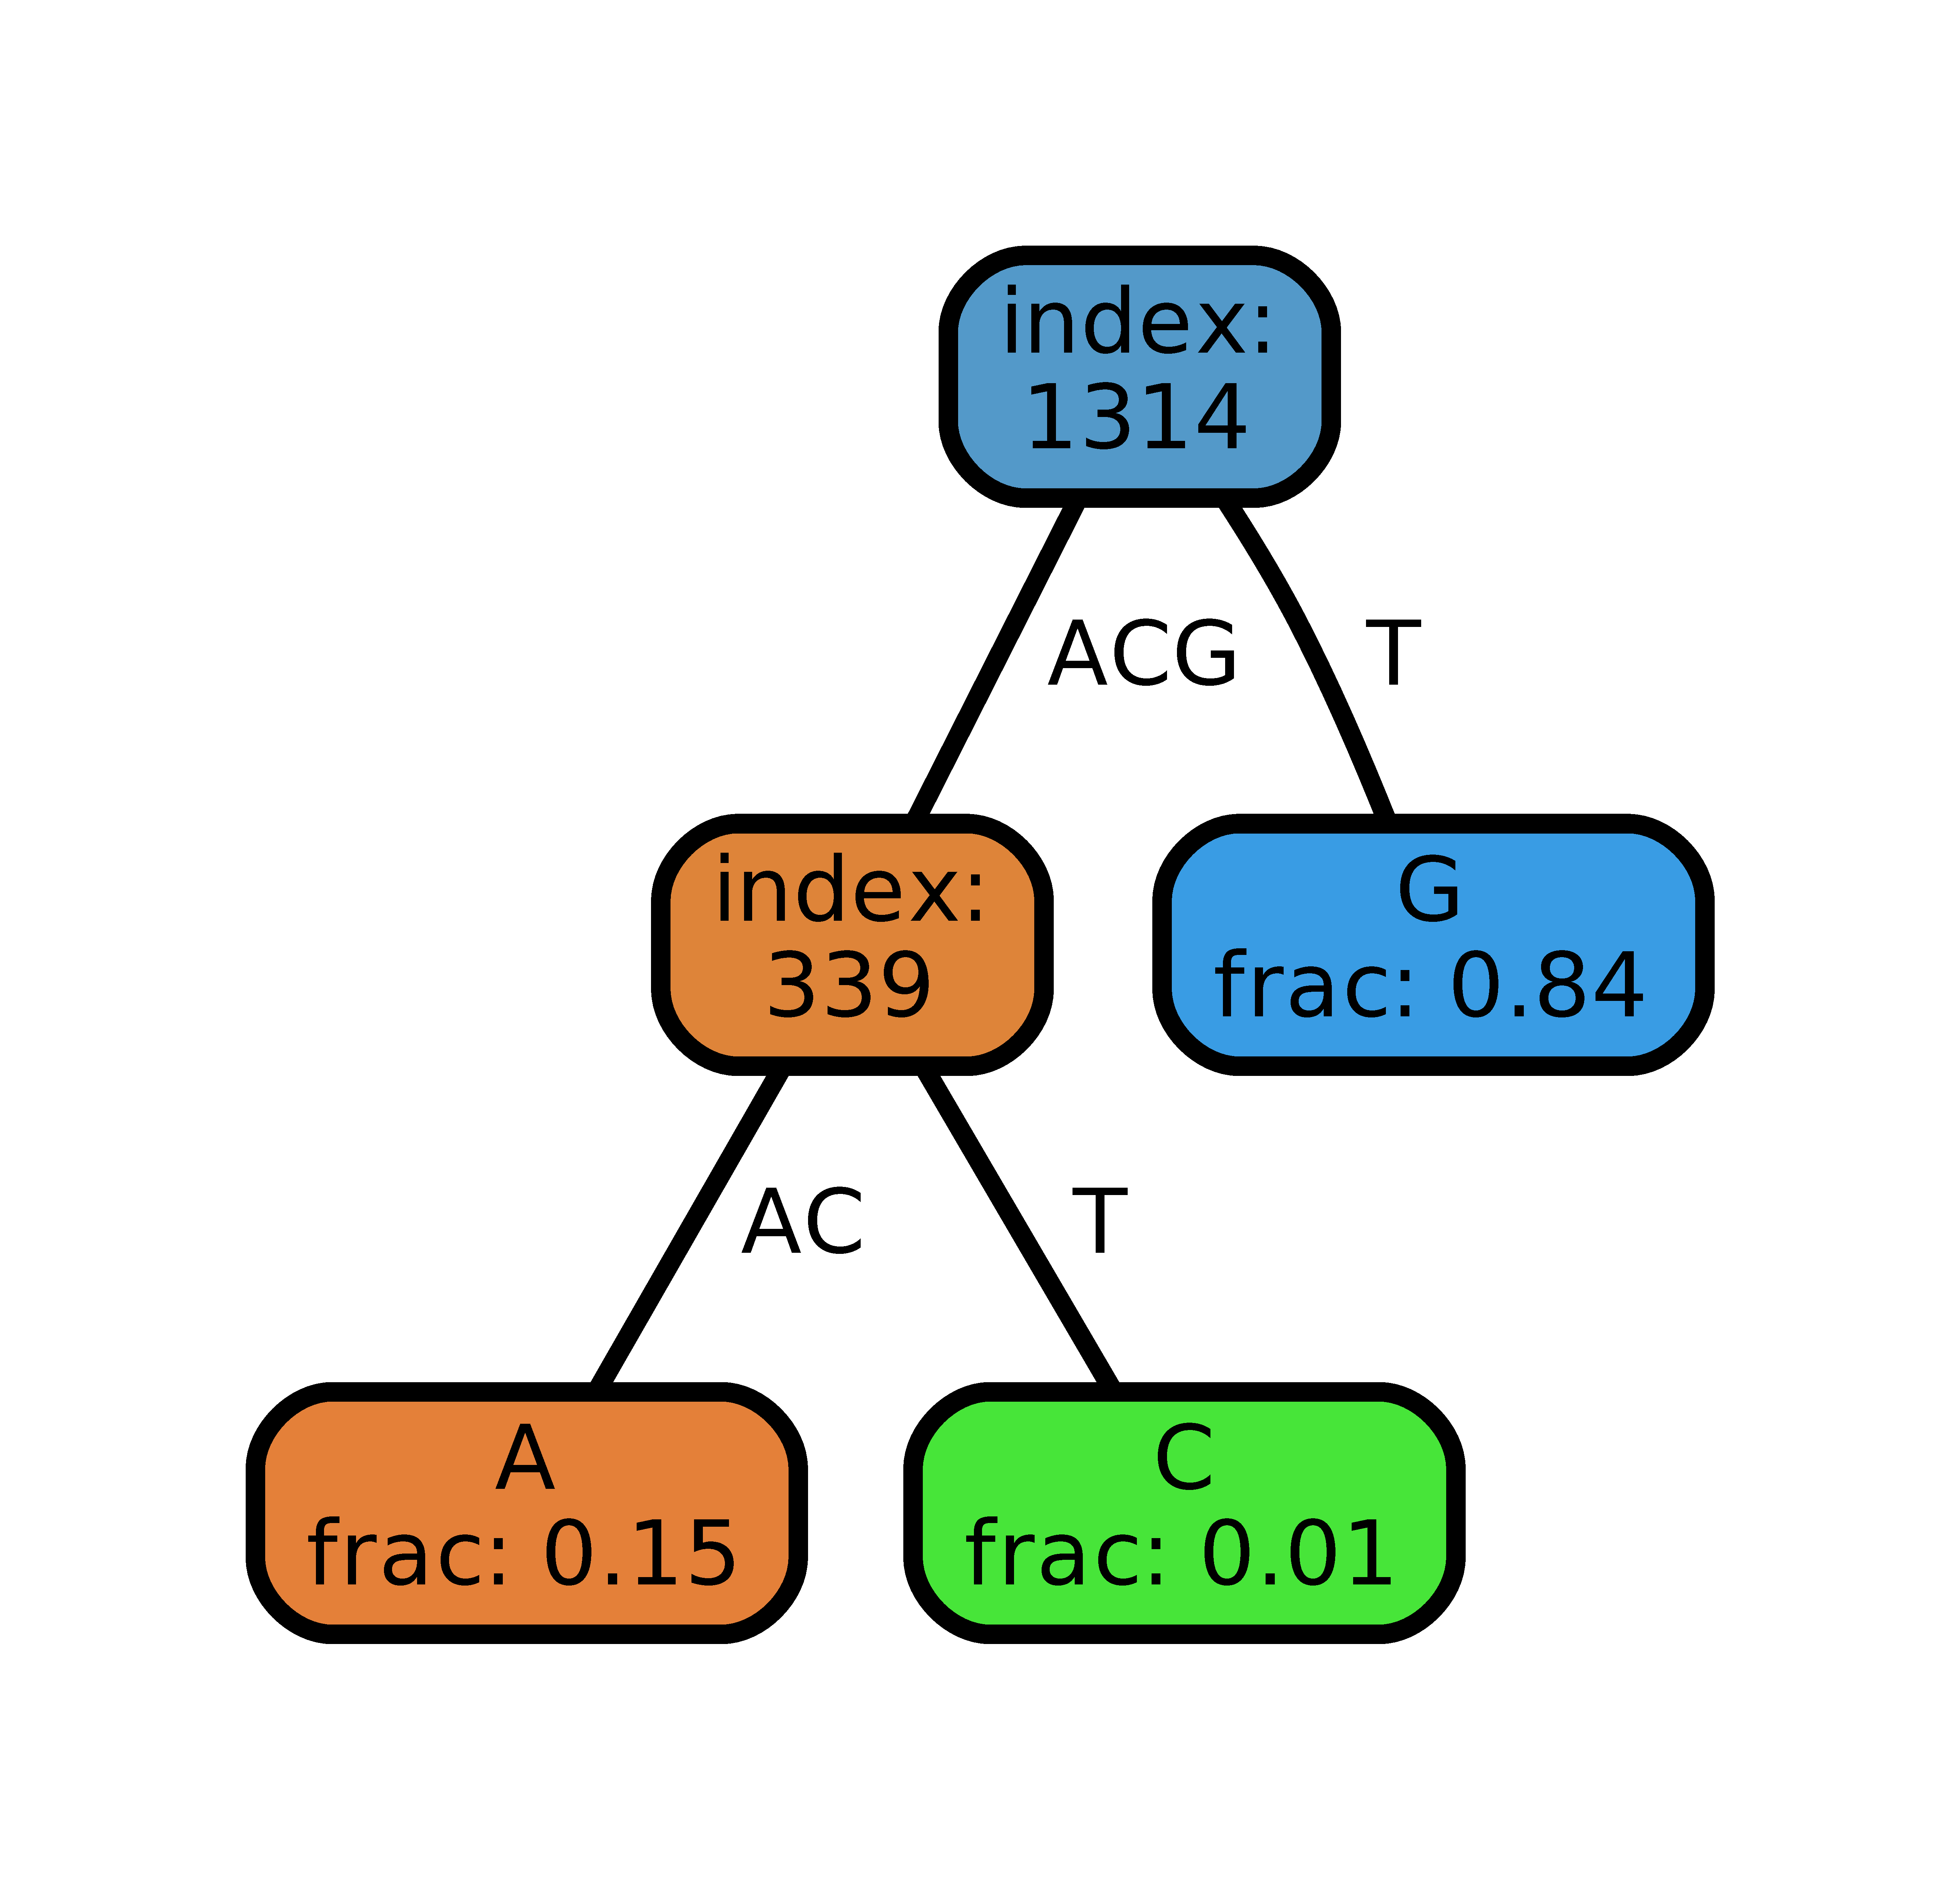
\includegraphics[width=\WDT]{Figures/trees/procP1064}};


\node[circle,inner sep=8pt,opacity=.5] (X1) at ([yshift=.57in,xshift=-.01in]P1274) {};
\draw [line width=4pt,\DCOLx,-latex,] (X1)  to [out=65,in=165,looseness=1]  (P1064);

\node[circle,inner sep=8pt,opacity=.5] (X2) at ([yshift=.57in,xshift=-.01in]P1263) {};
\draw [line width=4pt,\DCOLx,-latex,] (X2)  to [out=60,in=185,looseness=1]  (P1314);

\node[circle,inner sep=12pt,opacity=.5] (X3) at ([yshift=.57in,xshift=.15in]P1064) {};
\draw [line width=4pt,\DCOLx,-latex,] (X3)  to [out=0,in=-60,looseness=1]  (P1314);

\node[circle,inner sep=12pt,opacity=.5] (X4) at ([yshift=.87in,xshift=-.52in]P1314) {};
\draw [line width=4pt,\DCOLx,-latex,] (X4)  to [out=-180,in=80,looseness=1]  (P1263);

 \node[anchor=north,align=left,font=\bf\tt\footnotesize] (N3) at ([yshift=-6.1in,xshift=-1.85in]Z.south) {\bf\sffamily\fontsize{7}{8}\selectfont H1N1 2018\\\bf\sffamily\fontsize{7}{8}\selectfont Haemagglutinin Sequences\\GGAAAACAAAAGCAACAAAA$\cdots$TGA{\large\color{Red1} A}AAAAGA$\cdots$\\AGCAAAAGCAGGGGAAAACA$\cdots $GTT{\large\color{Red1}C}AACCAC$\cdots$\\AGCAAAAGCAGGGGAAAACA$\cdots$GTT{\large\color{Red1}T}AACCAC$\cdots$\\ATGAAGACTATCATTGCTTT$\cdots$ACC{\large\color{Red1}T}TGAGAA$\cdots$};

\node[anchor=west,align=left,font=\bf\sffamily\fontsize{8}{10}\selectfont,label={[font=\normalfont\itshape\sffamily,align=left,xshift=-.2in]90:$\bigstar$ mixed colors\\represent distributions}] (N4) at ([xshift=.2in,yshift=.05in]N3.east) {A/Italy/7366/2018\\
A/Baltimore/P0264/2018\\
A/Baltimore/P0278/2018\\  
A/Florida/61/2018};

\draw [ultra thick] ([yshift=.25in,xshift=.01in]N4.west) --++ (-.23in,-.190in);
\draw [ultra thick] ([yshift=.1in,xshift=.01in]N4.west) --++ (-.23in,-.2in);
 \draw [ultra thick] ([yshift=-0.05in,xshift=.01in]N4.west) --++ (-.23in,-.2in);
 \draw [ultra thick] ([yshift=-.2in,xshift=.01in]N4.west) --++ (-.23in,-.2in);

\draw [-{Latex[length=4mm]},ultra thick,line width=\LWD,Red1] ([xshift=0.55in,yshift=-.2in]N3.north) --++(0,.4in) node [yshift=-.95in,below,align=center,text=IndianRed2] {residue\\at index 1274};

\node[anchor=east,rounded corners=3pt,align=center] (I1) at ([yshift=-.4in,xshift=3.8in]P1274.west) {Color key$^\bigstar$};

\node[font=\bf\sffamily,anchor=north,rounded corners=3pt,text width=.1in,text height=.1in,fill=Purple1,align=center,opacity=\OPC] (I1) at ([yshift=-.05in]I1.south) {T};

\node[font=\bf\sffamily,anchor=north,rounded corners=3pt,text width=.1in,text height=.1in,fill=DarkOrange3!70,align=center,opacity=\OPC] (I1) at ([yshift=-.05in]I1.south) {A};

\node[font=\bf\sffamily,anchor=north,rounded corners=3pt,text width=.1in,text height=.1in,fill=SeaGreen2,align=center,opacity=\OPC] (I1) at ([yshift=-.05in]I1.south) {C};

\node[font=\bf\sffamily,anchor=north,rounded corners=3pt,text width=.1in,text height=.1in,fill=DodgerBlue2!80,align=center,opacity=\OPC] (I1) at ([yshift=-.050in]I1.south) {G};
\end{tikzpicture}};

\node [anchor=south west] (L1) at ([yshift=-.55in]T.north west) {\Large a.};
\node [anchor=south west] (L2) at ([yshift=-3.25in]T.north west) {\Large c.};
\node [anchor=south west] (L3) at ([yshift=-5.65in]T.north west) {\Large d.};

\end{tikzpicture}
